\documentclass{beamer}
%\usetheme{Ilmenau}
%\usecolortheme{beaver}

\usepackage[slovak,american]{babel}
\usepackage[utf8]{inputenc}
\usepackage{graphicx}
\usepackage{adjustbox}
 \usepackage{xcolor}
 
 \newsavebox\MBox
\newcommand\Cline[2][red]{{\sbox\MBox{$#2$}%
  \rlap{\usebox\MBox}\color{#1}\rule[-2.2\dp\MBox]{\wd\MBox}{1pt}}}

%\usefonttheme{serif}

\definecolor{UKOrange}{HTML}{ef9424} %
\definecolor{UKBrown}{HTML}{a96d5e} %
\definecolor{UKLight}{HTML}{d8b6ab} %
\definecolor{UKDark}{HTML}{7a4f44}
\definecolor{UKDarker}{HTML}{4d312b} 
\definecolor{UKDarkest}{HTML}{2e1e1a}
\definecolor{UKRed}{HTML}{bf1f1c}

\setbeamertemplate{footline}[frame number]{}
\setbeamertemplate{navigation symbols}{}

%\usecolortheme{beaver}
\setbeamertemplate{itemize item}[square]
\setbeamercolor{itemize item}{fg = UKBrown}
\setbeamercolor{itemize subitem}{fg = UKLight}
\setbeamercolor{enumerate item}{fg = UKDark}

\setbeamercolor{footnote}{fg=UKLight}
\setbeamercolor{footnote mark}{fg=UKLight}
\setbeamerfont{footnote}{size=\tiny}
\renewcommand\footnoterule{}

\usetheme{default}
\beamertemplatenavigationsymbolsempty
\setbeamercolor{title}{fg=white, bg=UKBrown}
\setbeamercolor{frametitle}{fg=white, bg=UKBrown}
\setbeamercolor{block title}{bg=UKBrown, fg= white}
\setbeamercolor{block body}{bg =UKLight, fg = UKDarkest}

\useoutertheme[subsection=false]{miniframes}
\AtBeginSection[]{\subsection{}}

\setbeamercolor{below lower separation line head}{bg=UKDark}
\addtobeamertemplate{headline}{}{%
  \begin{beamercolorbox}[colsep=0.5pt]{below lower separation line head}
  \end{beamercolorbox}
}
%\setbeamercolor*{mini frame}{fg=white,bg=UKRosy}
\setbeamercolor{section in head/foot}{fg=UKLight, bg=UKDark}

%\setbeamertemplate{itemize/enumerate body begin}{\normalsize}
%\setbeamertemplate{itemize/enumerate subbody begin}{\normalsize}




%\newcommand{\codeblock}[2]{ \begin{block}{#1} \begin{verbatim}#2\end{verbatim}\end{block}}

%\defbeamertemplate*{title page}{customized}[1][]
%{
%  \begin{centering}
%    \begin{beamercolorbox}[sep=8pt,center]{title}
%      \usebeamerfont{title}\inserttitle
%    \end{beamercolorbox}
%  \end{centering}
%  \bigskip
%
%\begin{columns}[onlytextwidth,T]
%
%
%  \column{27mm}
%  \includegraphics[width=27mm]{images/logoFMFI.png}
%  
%  \column{\dimexpr\linewidth-54mm-6mm}
%  \centering
%  \vspace{5mm}  
%  \usebeamerfont{author}\insertauthor\par
%  \vspace{5mm}
%  \usebeamerfont{institute}\insertinstitute\par
%
%  \column{27mm}
%  \includegraphics[width=27mm]{images/logoUK.png}  
%\end{columns}
%\centering
%\vspace{7mm}
%  \usebeamerfont{date}\insertdate\par
%}


\title[Výber príznakov]{Rozpoznávanie obrazcov - 4. cvičenie \\ Výber príznakov}
\author[Viktor Kocur]{Viktor Kocur \\{\small viktor.kocur@fmph.uniba.sk}}
\institute{DAI FMFI UK}
\date{10.3.2020}
%\titlegraphic{\includegraphics[width=2.7cm]{images/logoFMFI.png}\hspace*{1cm}~%
%   \includegraphics[width=2.7cm]{images/logoUK.png}
%}



\begin{document}
\selectlanguage{slovak}

\begin{frame}[plain]
  \titlepage  
\end{frame}

\section{Informačno-teoretické miery}

\begin{frame}
\frametitle{Entrópia}
  \centering
  Shannonvá entrópia
  \begin{equation*}
  H(Y) = - \sum_{y \in \omega} P(Y = y) \cdot log_2(P(Y = y)) 
  \end{equation*}
  

\begin{columns}[onlytextwidth,T]


  \column{27mm}
  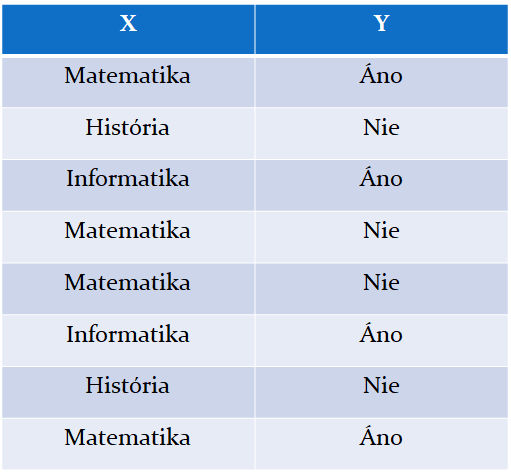
\includegraphics[width=60mm]{tabulka.png}
  
  \column{\dimexpr\linewidth-60mm-6mm}

  \begin{itemize}
  \item<2-> $H(X) = 1.5$
  \item<3-> $H(Y) = 1$
  \end{itemize}
\end{columns}
\end{frame}



\begin{frame}
\frametitle{Entrópia}
  \centering
  Špecifická podmienená entrópia
  \begin{equation*}
  H(Y| X = v) = H(Y), \textnormal{len pre hodnoty} Y, \textnormal{kde } X = x 
  \end{equation*}  

\begin{columns}[onlytextwidth,T]


  \column{27mm}
  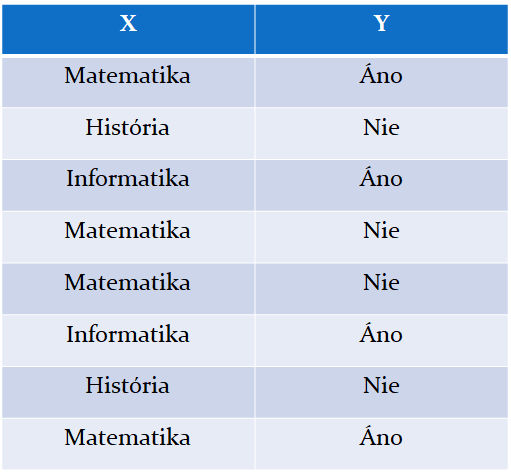
\includegraphics[width=60mm]{tabulka.png}
  
  \column{\dimexpr\linewidth-60mm-6mm}

  \begin{itemize}
  \item<2-> $H(Y| X = M) = 1$
  \item<3-> $H(Y| X = H) = 0$
  \item<4-> $H(Y| X = I) = 0$
  \end{itemize}
\end{columns}
\end{frame}


\begin{frame}
\frametitle{Entrópia}
  \centering
  Podmienená entrópia
  \begin{equation*}
  H(Y| X) = \sum_{x \in \Omega_x} P(X = x) \cdot H(Y | X = x)
  \end{equation*}  

\begin{columns}[onlytextwidth,T]


  \column{27mm}
  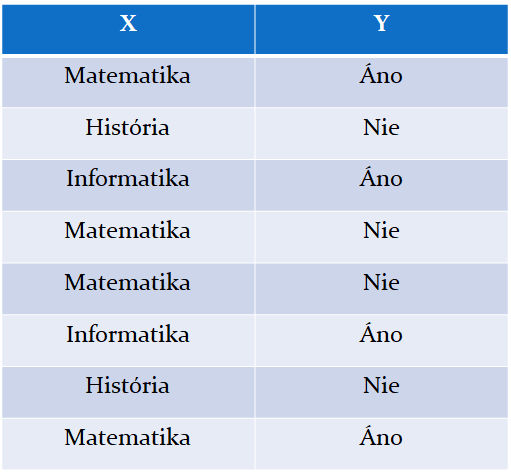
\includegraphics[width=60mm]{tabulka.png}
  
  \column{\dimexpr\linewidth-60mm-6mm}

  \begin{itemize}
  \item<2-> $H(Y|X) = 0.5$
  \end{itemize}
\end{columns}
\end{frame}



\begin{frame}[fragile]
\frametitle{Entrópia - Matlab}
\begin{block}{Načítanie dát}
\begin{verbatim}
load census1994
Y = categorical(adultdata.salary);
X1 = categorical(adultdata.education);
\end{verbatim}
\end{block}

\begin{block}{Úloha}
Vytvorte funkciu entropia(X), ktorá vráti hodnotu ktorú sme definovali ako $H(X)$.
\end{block}

\begin{block}{countcats}
countcats(X) - vráti početnosti jednotlivých kategórii z X (ak je X typu categorical)
\end{block}
\end{frame}


\begin{frame}
\frametitle{Entrópia - Matlab}

\begin{block}{Úloha}
Vytvorte funkciu podm\_entropia(Y, X), ktorá vráti hodnotu ktorú sme definovali ako $H(Y|X)$.
\end{block}

\begin{block}{categories}
c = categories(X) - vráti cell štruktúru c s jednolivými kategóriami z X (ak je X typu categorical).  Pozn.: z cell dostane kategóriu ako c\{i\} a použijeme pri indexácii logickou maticou (X == c\{i\}).
\end{block}
\end{frame}


\end{document}